\chapter{Steekproefonderzoek}
Een reden om kwantitatief onderzoek uit te voeren is het kunnen doen van uitspraken die een representatief beeld van de werkelijkheid geven. Hierbij wordt vaak gebruikgemaakt van een steekproef. Een steekproef is een selectie uit een totale populatie ten behoeve van een meting van bepaalde eigenschappen van die populatie.

\begin{figure}
\centering
  \begin{tikzpicture}[xscale=4,yscale=2]
    \draw (0,2) -- (0,0);
    \foreach \num/\label in {0/0, 0.2/20, .4/40, .6/60, .8/80, 1/100, 1.2/120, 1.4/140, 1.6/160, 1.8/180, 2/200}{%
      \draw (0, \num) -- (2.5, \num);
      \draw[shift={(0, \num)}] (1pt,0pt) -- (-1pt,0pt) node[left] {\scriptsize \label};
    }

    \node[anchor=north] (hero1) at (0.3,1.5)
    {
\includegraphics[height=2.9cm]{images/les2-hero-1}};
    \node[anchor=north] (hero2) at (0.8,2.05)
    {
\includegraphics[height=4cm]{images/les2-hero-2}};
    \node[anchor=north] (hero3) at (1.3,1.575)
    {
\includegraphics[height=3.1cm]{images/les2-hero-3}};
    \node[anchor=north] (hero4) at (1.8,2.1)
    {
\includegraphics[height=4.1cm]{images/les2-hero-4}};
    \node[anchor=north] (hero5) at (2.3,1.95)
    {
\includegraphics[height=3.8cm]{images/les2-hero-5}};

    \node (size1) at (0.3, 1.5) {\scriptsize 141 cm};
    \node (size2) at (0.8, 2.1) {\scriptsize 198 cm};
    \node (size3) at (1.3, 1.51) {\scriptsize 143 cm};
    \node (size4) at (1.8, 2.15) {\scriptsize 201 cm};
    \node (size5) at (2.3, 1.95) {\scriptsize 184 cm};
  \end{tikzpicture}
  \caption{De superhelden die we onderzoeken}
  \label{fig:superheldenSteekproef}
\end{figure}

\begin{figure}
  \centering
  
\includegraphics[width=0.85\textwidth]{images/les5-heroes.jpg}
  \caption{Onze superhelden die we onderzoeken vormen een steekproef uit de populatie van alle superhelden.}
  \label{fig:populatieHelden}
\end{figure}

\section{Populatie en Steekproeven}
\begin{definition}[Populatie]
  De verzameling van \textbf{alle} objecten of personen waar men in ge\"interesseerd is en onderzoek naar wil doen noemt men de \index{populatie} populatie. Een ander woord is ook wel onderzoeksgroep of doelgroep.
\end{definition}

\begin{definition}[Steekproef]
  Wanneer met een subgroep uit een populatie gaat onderzoeken, dan noemen we die groep een \index{steekproef} steekproef.
\end{definition}

\begin{definition}[Steekproefkader]
  Een \index{steekproefkader} steekproefkader is een lijst van alle leden van een te onderzoeken populatie.
\end{definition}

Er zijn een aantal redenen waarom een steekproef genomen wordt:
\begin{itemize}
  \item Populatie is te groot om een volledig onderzoek te doen.
  \item Kostbare metingen waardoor het onderzoek te duur wordt.
  \item Wanneer snelheid belangrijk is, is het vaak sneller een subgroep te onderzoeken;
  \item Gemakkelijker \dots
\end{itemize}

Om een steekproef op te zetten volg je volgende stappen:
\begin{enumerate}
  \item \textbf{Definitie populatie}: Wie is er deel van de populatie? Dit hangt nauw samen met de probleemstelling van het onderzoek. Dit is een zeer belangrijke stap waar je niet licht over mag gaan. Elementen die van belang zijn, zijn bijvoorbeeld sociale, demografische of fysieke kenmerken zoals geslacht, leeftijd, woonplaats \dots
  \item \textbf{Bepalen van steekproefkader}: Een populatie heeft verschillende segmenten zoals bijvoorbeeld rijke superhelden, arme superhelden, bekende en onbekende superhelden, superhelden met en zonder oudercomplex \dots In de praktijk is het meestal onmogelijk om de populatie als geheel te onderzoeken. Daarom beperken we ons vaak tot enkele redelijk homogene subpopulaties of segmenten. De populatiesegmenten die daadwerkelijk onderzocht worden noemen we de operationele populatie.
  \item \textbf{Budget en Tijd}: het aantal te onderzoeken objecten of personen zal ook afhankelijk zijn van budget en tijd.
\end{enumerate}

\section{Kiezen van steekproefmethode}
  Soms is de populatie die men wenst te bestuderen erg verschillend op een aantal belangrijke kenmerken. Daartoe wordt de populatie als geheel in een aantal elkaar niet-overlappende en homogene strata of klassen ingedeeld.

\begin{definition}[Gestratificeerde steekproef]
Een \textbf{gestratificeerde} \index{gestratificeerd} steekproef is proportioneel als het aandeel van de subpopulatie in de steekproef gelijk is aan het aandeel van de subpopulatie in de populatie als geheel.
\end{definition}

\begin{example}
  Indien we uit een populatie van de superhelden kijken naar de leeftijd van  mannen en vrouwen, zien we in tabel \ref{tab:heldenPopulatie1} de absolute waarden. We kunnen niet alle superhelden ondervragen, maar indien we een steekproef nemen waarbij de mannen en leeftijdscategorie\"en relatief equivalent zijn met de populatie, hebben we een gestratificeerde steekproef genomen (zie tabel \ref{tab:heldenPopulatie2}).
\end{example}

  \begin{table}
  \centering
    \begin{tabular}{l|cccc|c}
      & \multicolumn{4}{c|}{\textbf{Leeftijd}} & \\
      Geslacht & $\le 18$ & $]18,25]$ & $]25, 40]$ & $> 40$ & Totaal\\
      \hline
      Vrouw & 500 & 1500 & 1000 & 250 & 3250 \\
      Man   & 400 & 1200 & 800 & 160 & 2560\\
      \hline
      Totaal & 900 & 2700 & 1800 & 410 & 5810
    \end{tabular}
    \caption{Frequenties van de superhelden in de populatie volgens geslacht en leeftijdscategorie}
    \label{tab:heldenPopulatie1}
\end{table}

\begin{table}
  \centering
    \begin{tabular}{l|cccc|c}
      & \multicolumn{4}{c|}{\textbf{Leeftijd}} & \\
      Geslacht & $\le 18$ & $]18,25]$ & $]25, 40]$ & $> 40$ & Totaal\\
      \hline
      Vrouw & 50 & 150 & 100 & 25 & 325 \\
      Man   & 40 & 120 & 80 & 16 & 256\\
      \hline
      Totaal & 90 & 270 & 180 & 41 & 581
    \end{tabular}
      \caption{Steekproef van superhelden gestratificeerd volgens geslacht en leeftijdscategorie.}
    \label{tab:heldenPopulatie2}
  \end{table}

Nadat gestratificieerd is, moet bepaald worden op welke wijze binnen ieder stratum het aantal benodigde objecten of respondenten gekozen moet worden. Bij de toevals- of \textbf{aselecte} \index{aselect} steekproeven heeft elk element van de populatie een even mogelijke kans om in de steekproef te worden opgenomen. Dit heeft als gevolg dat je op basis van de data van een aselecte steekproef conclusies kan trekken ten aanzien van de kenmerken van een populatie, en dit in tegenstelling met een \textbf{niet-aselecte} steekproef. In een niet-aselecte steekproef kent men de kans niet dat elk lid van de populatie heeft om in de steekproef terecht te komen, met als gevolg dat je gegevens enkel gelden voor je onderzochte groep.

\subsection{Fouten bij steekproeven}
\subsubsection{Toevallige steekproeffouten}
Wanneer er puur door het toeval een verschil is in een waarde voor de populatie en de steekproef.

\subsubsection{Systematische steekproeffouten}
Een procedure in de steekproef die een fout oplevert die een systematische oorzaak heeft en dus niet te wijten is aan toevallige effecten. Bijvoorbeeld door systematisch een bevoordeeld deel van de populatie te ondervragen. Als we onze superhelden zouden ondervragen via het internet, sluiten we alle superhelden uit die geen internetverbinding hebben.

\subsubsection{Toevallige niet-steekproeffouten}
Hieronder vallen bijvoorbeeld verkeerd aangekruiste antwoorden of verschil in interpretatie van de vragen.

\subsubsection{Systematische niet-steekproeffouten}
Wanneer bijvoorbeeld respondenten met een sterke band met het onderzoek eerder geneigd zijn om een vragenlijst in te vullen, ga je positievere antwoorden krijgen - terwijl ze niet representatief zijn voor de gehele populatie.

\subsection{Aanpassing formules standaarddeviatie}
We noemen het gemiddelde van de steekproef het steekproefgemiddelde en gebruiken hiervoor het symbool $\overline{x}$ (dit hebben we stilzwijgend al een aantal keer gedaan in de vorige hoofdstukken).

Als we de standaardafwijking van een steekproef willen bepalen dan moeten we niet meer delen door $n$ (aantal metingen) maar door $(n-1)$. Waarom?

Aangezien de som van de afwijkingen $x_{i} - \overline{x}$ steeds 0 oplevert (zie hieronder in vergelijking \ref{eq:sumGemid}), kan de laatste afwijking gevonden worden uit de eerste $n-1$ afwijkingen. We berekenen dus niet het gemiddelde van $n$ getallen zonder verwantschap. Slecht $n-1$ van de gekwadrateerde afwijkingen kunnen vrij bewegen, daarom berekenen we het gemiddelde door het totaal te delen door $n-1$. Het getal $n-1$ noemt men het aantal vrijheidsgraden van de variantie of van de standaardafwijking.

\begin{equation}
 \sum_{i}^{n}(x_{i} - \overline{x}) = \sum_{i}^{n}x_{i} - \sum_{i}^{n}\overline{x} = \sum_{i}^{n}x_{i} - n (\frac{1}{n}\sum_{i}^{n} x_{i})
\label{eq:sumGemid}
\end{equation}

\section{Kansverdeling van een steekproef}
\subsection{Stochastisch experiment}
Een random (of stochastisch) experiment heeft volgende elementen nodig:

\begin{definition}[Universum of Uitkomstenruimte]\
 Het universum of uitkomstenruimte van een experiment
is de verzameling van alle mogelijke uitkomsten van dit experiment en
wordt genoteerd met $\Omega$.
\end{definition}
~\\
\textbf{Opmerkingen}
\begin{itemize}
\item De uitkomstenruimte moet \emph{volledig}\/ zijn: elke mogelijke
uitkomst van een experiment moet tot $\Omega$ behoren.
\item Bovendien moet elke
uitkomst van een experiment overeenkomen met \emph{juist \'e\'en}\/ element van
$\Omega$.
\item Samengevat: na het uitvoeren van een experiment is het  mogelijk  om eenduidig
aan te geven welk element van $\Omega$ zich heeft voorgedaan.
\end{itemize}

\begin{definition}[Gebeurtenis]
 Een gebeurtenis is een deelverzameling van de uitkomstenruimte. Een enkelvoudige of elementaire gebeurtenis is een singleton;   een samengestelde gebeurtenis heeft cardinaliteit groter dan 1.
\end{definition}
Gebeurtenissen die geen gemeenschappelijke uitkomsten hebben noemt men
{disjunct. \\
Disjuncte gebeurtenissen kunnen dus nooit samen voorkomen.\\
Wanneer de gebeurtenissen $A$ en $B$ disjunct zijn dan geldt
$A \cap B = \emptyset$.
Startend met
 de gebeurtenissen $A$ en $B$ kan men de volgende gebeurtenissen vormen:
 \begin{itemize}
  \item $A$ \textbf{of} $B$, of wiskundig genoteerd $A \cup B$;
  \item $A$ \textbf{en} $B$, of wiskundig genoteerd $A \cap B$;
  \item \textbf{niet} $A$, of wiskundig genoteerd $\overline{A}$.
\end{itemize}
\textbf{Opmerkingen}
\begin{itemize}
\item Door inductie leidt men gemakkelijk  af dat
de unie van $n$  gebeurtenissen $A_1$ t.e.m.~$A_n$ eveneens
een gebeurtenis is.
\item Idem voor de doorsnede van
gebeurtenissen.
\item Voor sommige toepassingen is het nodig om ook (aftelbaar) oneindige
unies en doorsnedes te beschouwen.
\end{itemize}

\begin{definition}[Kansruimte]
Het toekennen van kansen aan gebeurtenissen dient aan de volgende drie regels te voldoen.
\begin{enumerate}
\item Kansen zijn steeds positief:
 $P(A) \geq 0$ voor elke $A$.
  \item
  De uitkomstenruimte heeft kans 1:
  $P(\Omega) = 1.$
 \item Wanneer $A$ en $B$ \emph{disjuncte}\/ gebeurtenissen zijn dan is
 \[P(A\cup B) = P(A) + P(B). \]
 Dit noemt men de somregel.
\end{enumerate}
Wanneer de functie $P$ aan de bovenstaande eigenschappen (axioma's) voldoet
dan noemt men het drietal $(\Omega, \mathcal{P}(\Omega), P)$ een
kansruimte (met $\mathcal{P}(\Omega)$ de \emph{machtsverzameling} van $\Omega$, d.w.z.~de verzameling van alle deelverzamelingen van $\Omega$).
\end{definition}

\begin{example}
Beschouw een uitkomstenruimte $\Omega =  \left\{ 1,2,3,4,5,6 \right\} $ en
een kansfunctie $P(\omega)=\frac{1}{|\Omega|}$, dan zou dit een dobbelsteen
kunnen voorstellen met uitkomsten 1 tot en met 6 met een kans
$P(\omega) = \frac{1}{6}$ om een van de nummers te werpen.
\end{example}

In dit onderdeel van de  cursus gaan we ons bezig houden met \textbf{inductieve statistiek}: op basis van een getrokken steekproef uitspraken doen over de populatie.

\subsection{Kansverdeling}
\subsubsection{Discrete kansverdeling}
Als we het voorbeeld nemen van het gooien van een dobbelsteen, dan kunnen we de kans dat we een van de getallen $\Omega = \{1,2,3,4,5,6\}$ in een tabel zetten of kunnen er een histogram van maken.  Er zijn een aantal belangrijke opmerkingen hierbij:
\begin{enumerate}
  \item De kansen zijn allemaal groter of gelijk aan nul.
  \item De kans op een getal is gelijk aan de bijbehorende oppervlakte van de staaf.
  \item De totale oppervlakte van alle staven is 1.
\end{enumerate}

Een ander voorbeeld is het gooien van twee dobbelstenen met de mogelijke uitkomst. Je hebt volgens de productregel $6 \times 6 = 36$ mogelijke uitkomsten. Om bijvoorbeeld drie te gooien heb je twee mogelijkheden (kans $P(X=3) = \frac{2}{36}$). Zie voor de andere getallen tot en met 7 de tabel ($ P[X=n] = \frac{n-1}{36}$).

Als we dit nu in een histogram steken bekomen we een mooie trap naar boven tot 7 en dan weer naar beneden. Nu kan je makkelijk zien dat:
\begin{itemize}
  \item Voor de kans om 10 of meer te gooien moet je bijvoorbeeld die blauwe oppervlakte hebben.
  \item Voor de kans op een aantal meer dan 2 maar minder dan 7 moet je de rode oppervlakte hebben.
  \item Voor de kans op een aantal meer dan 7 maar minder dan 10 moet je de groene oppervlakte hebben.
  \item Dan is het ook logisch dat de totale oppervlakte 1 is: de kans dat 1 van al die mogelijkheden voorkomt is natuurlijk 100\%.
\end{itemize}

\subsubsection{Continue kansverdeling}

Continue kansverdelingen zijn verdelingen waarbij hetgeen we meten niet alleen een beperkt aantal waarden kan aannemen (nominaal en ordinaal meetniveau), maar ook alle er tussenliggende waarden (ratio- en intervalniveau). Neem bijvoorbeeld het gewicht van onze superhelden. Dat is continu, immers dat kan niet alleen $60$ of $70$ kilo zijn, maar ook (bij benadering)  $66,8735485653$ kilo. In principe zijn alle tussenliggende waarden mogelijk (al is dat in praktijk vaak niet te meten). Dat heeft een belangrijk gevolg voor de kansverdeling. Die bestaat nu (in theorie) niet meer uit losse staafjes, maar is een vloeiende kromme geworden. Dat betekent dat de kans op bijvoorbeeld precies $70$ kilogram een kans nul heeft. Bij precies $70$ kg hoort een verticaal lijntje, en een lijntje heeft oppervlakte nul. Nu is die kans natuurlijk ook nul. Als we zeggen $70$ kg, dan bedoelen we meestal tussen $69,5$ en $70,5$, of preciezer het interval $[69,5; 70,5[$. Als we zeggen $70,00000$ kg, dan bedoelen we iets als binnen $[70,000005; 69,999995[$ kg.

De twee regels voor kansverdelingen hierboven blijven gewoon geldig. Als zo'n kromme een goede kansverdeling is, dan moet de totale oppervlakte ervan 1 zijn, en dan kun je de kans op een gewicht dat bijvoorbeeld tussen de 60 en 70 kg ligt uitrekenen door de oppervlakte hiernaast te bepalen (merk op dat het uiteindelijk niet belangrijk is of die $60$ en $70$ zelf ook nog tot het interval behoren, die hebben toch kans nul!).

\section{De normale verdeling}

\begin{figure}[t]
\centering
\begin{tikzpicture}
\begin{axis}[
  domain=0:10, samples=100,
  axis lines*=left, xlabel=$x$, ylabel=$y$,
  every axis y label/.style={at=(current axis.above origin),anchor=south},
  every axis x label/.style={at=(current axis.right of origin),anchor=west},
  height=5cm, width=12cm,
  xtick={5,3.5,6.5}, ytick=\empty,
  enlargelimits=false, clip=false, axis on top,
  grid = major
  ]
  \addplot [fill=cyan!20, draw=none, domain=0:9] {gauss(5,1.5)} \closedcycle;
  \draw [yshift=-0.6cm, latex-latex](axis cs:3.5,0) -- node [fill=white] {$\sigma$} (axis cs:6.5,0);
\end{axis}
\end{tikzpicture}
\caption{De kansverdeling van de reactiesnelheid van superman. Deze grafiek noemen we de normaalverdeling met gemiddelde $\mu = 5$ ms en standaarddeviatie $\sigma = 1,5 ms.$}
\label{fig:verdelingReactievermogen}
\end{figure}


In figuur \ref{fig:verdelingReactievermogen} tonen we de kansverdeling van de reactiesnelheid X van superman. Deze grafiek noemen we de normaalverdeling met gemiddelde 5 ms en standaarddeviatie 1,5 ms. Symbolisch:
\[ X  \sim Nor(\mu = 5; \sigma = 1,5) \]

De functie die hiermee gepaard gaat is de volgende:

\begin{equation}
  f(x) = \frac{1}{\sigma \sqrt{2\pi}} e^{-\frac{1}{2} \frac{(x - \mu)^{2}}{\sigma^{2}}}
  \label{eq:normalFunction}
\end{equation}

De normale verdeling kent volgende eigenschappen:
\begin{itemize}
  \item Normale verdeling is klokvormig
  \item De normale verdeling is symmetrisch
  \item Vanwege symmetrie is gemiddelde, mediaan en modus aan elkaar gelijk
  \item De totale oppervlakte onder de klokvormige figuur is 1
  \item In gebied $\sigma$ onder $\mu$ en $\sigma$ boven $\mu$ (het zogenoemde sigma gebied) ligt ongeveer 68\% van de waarnemingen.
  \item In het gebied $2\sigma$ boven en onder $\mu$ ligt ongeveer 95\% van alle waarnemingen.
  \item Voor de verschillende gebieden zie figuur \ref{fig:standaardNormaleVerdeling}
\end{itemize}

\subsection{De standaardnormale verdeling}

Indien de toevalsveranderlijke $X \sim N(\mu,\sigma)$ verdeeld is dan is de toevalsvariabele $Z = \frac{X - \mu}{\sigma}$ normaal verdeeld: $Z \sim N(0,1)$. Dit noemen we de standaardnormale verdeling.

  % Bron: http://johncanning.net/wp/?p=1202
  \begin{center}
  \begin{figure}
  \centering
    \begin{tikzpicture}
      \begin{axis}[
          no markers, domain=0:10, samples=100,
          axis lines*=left,height=6cm, width=10cm,
          xtick={-3, -2, -1, 0, 1, 2, 3}, ytick=\empty,
          enlargelimits=false, clip=false, axis on top,
          grid = major
        ]
        \addplot [smooth,fill=cyan!20, draw=none, domain=-3:3] {gauss(0,1)} \closedcycle;
        \addplot [smooth,fill=orange!20, draw=none, domain=-3:-2] {gauss(0,1)} \closedcycle;
        \addplot [smooth,fill=orange!20, draw=none, domain=2:3] {gauss(0,1)} \closedcycle;
        \addplot [smooth,fill=blue!20, draw=none, domain=-2:-1] {gauss(0,1)} \closedcycle;
        \addplot [smooth,fill=blue!20, draw=none, domain=1:2] {gauss(0,1)} \closedcycle;
        \addplot[<->] coordinates {(-1,0.4) (1,0.4)};
        \addplot[<->] coordinates {(-2,0.3) (2,0.3)};
        \addplot[<->] coordinates {(-3,0.2) (3,0.2)};
        \node[coordinate, pin={68.2\%}] at (axis cs: 0, 0.35){};
        \node[coordinate, pin={95\%}] at (axis cs: 0, 0.25){};
        \node[coordinate, pin={99.7\%}] at (axis cs: 0, 0.15){};
        \node[coordinate, pin={34.1\%}] at (axis cs: -0.5, 0){};
        \node[coordinate, pin={34.1\%}] at (axis cs: 0.5, 0){};
        \node[coordinate, pin={13.6\%}] at (axis cs: 1.5, 0){};
        \node[coordinate, pin={13.6\%}] at (axis cs: -1.5, 0){};
        \node[coordinate, pin={2.1\%}] at (axis cs: 2.5, 0){};
        \node[coordinate, pin={2.1\%}] at (axis cs: -2.5, 0){};
      \end{axis}
    \end{tikzpicture}
    \caption{De standaardnormale verdeling met opdeling in zones}
    \label{fig:standaardNormaleVerdeling}
    \end{figure}
  \end{center}

In het algemeen kan dus bij een waarneming $x$ de zogenaamde $z$-score bepalen als volgt:

\begin{equation}
  z = \frac{x-\mu}{\sigma}
  \label{eq:zscore}
\end{equation}

Deze score geeft dus aan hoe extreem een waarneming is of anders gezegd, hoeveel standaarddeviaties is de waarneming $x$ van het gemiddelde $\mu$ verwijderd. Voor een willekeurige $x$-waarde kunnen we met formule \ref{eq:zscore} de bijhorende $z$-score bepalen. Voor deze $z$-scores heeft men tabellen opgesteld met de kansen dat een waarde kleiner dan $z$ getrokken wordt uit Z, de zgn.~linkerstaartkans\footnote{Er bestaan ook tabellen met de rechterstaartkans}: $P(Z<z)$.

R heeft eveneens functies voor het rekenen met kansen van normaal verdeelde variabelen. Deze worden samengevat in Tabel~\ref{rab:norm-prob-r}.

\begin{table}
  \centering
  \begin{tabular}{ll}
  	\textbf{Functie}      & \textbf{Betekenis}                                             \\ \hline
  	\verb|pnorm(x, m, s)| & Linkerstaartkans, $P(X<\mathtt{x})$                            \\
  	\verb|dnorm(x, m, s)| & Hoogte van de Gausscurve op punt \texttt{x}                    \\
  	\verb|qnorm(p, m, s)| & Onder welke grens zal \texttt{p}\% van de waarnemingen liggen? \\
  	\verb|rnorm(n, m, s)| & Genereer \texttt{n} normaal verdeelde random getallen
  \end{tabular}
  
  \caption{Kansberekeningsfuncties in R voor een normale verdeling met gemiddelde \texttt{m} en standaardafwijking \texttt{s}. Indien argumenten \texttt{m} en \texttt{s} weglaten worden, wordt de standaardnormaalverdeling verondersteld.}
  \label{rab:norm-prob-r}
\end{table}

We komen dan tot de volgende methode voor het berekenen van kansen met de normale verdeling:
\begin{enumerate}
  \item Bepaal de kansvariabele met de bijbehorende normale verdeling
  \item Bereken de $z$-score bij de bijhorende $x$-waarde.
  \item Schets de plaats van de gevraagde kans
  \item Herleid de gevraagde kans met behulp van de schets tot een linkerstaartkans en gebruik de $z$-tabel van de standaardnormale verdeling om deze te bepalen. Gebruik indien nodig de symmetrieregel en de regel van 100\% kans.
\end{enumerate}

\begin{example}
Hoe groot is de kans dat superman in minder dan 4 ms reageert?
\[ P(X < 4) = P(Z < -0,67) = 0,2514 \]
\end{example}
\begin{example}
Hoe groot is de kans dat hij in minder dan 7 ms reageert?
\[ P(X < 7) = P(Z < 1,33) = 0,9082 \]
\end{example}
\begin{example}
Hoe groot is de kans dat superman in minder dan 3 ms reageert?
\[ P(X<3) = P(Z < -1,33) = 0,0918 \]
\end{example}
\begin{example}
Hoe groot is de kans dat hij reageert tussen de 2 en 6,5 ms
\[ P( 2 < X < 6,5) = P(X<6,5) - P(X<2) = P(Z<1) - P(Z<-2) = 0,8186 \]
\end{example}

\subsection{Testen op normaliteit}

Er zijn verschillende methoden die kunnen gebruikt worden om na te gaan of een steekproef uit een normale verdeling komt.
\begin{enumerate}
  \item Construeer een histogram voor de gegevens en bekijk de vorm van de grafiek. Als de gegevens bij benadering een normale verdeling hebben, zal de vorm van het histogram een klokcurve vormen.
  \item Bereken de intervallen $\overline{x} \pm s$, $\overline{x} \pm 2s$, $\overline{x} \pm 3s$ en bepaal het percentage meetwaarden dat binnen elk van deze intervallen valt. Als de gegevens ongeveer normaal verdeeld zijn, zullen de percentages ongeveer gelijk zijn aan respectievelijk 68\%, 95\% en 99,7\%.
  \item Construeer een QQ-plot (normaliteitsplot, zie Definitie~\ref{def:qq-plot}) voor de gegevens. Als de gegevens ongeveer normaal verdeeld zijn, zullen de punten ongeveer op een rechte lijn liggen.
  \item Bereken de \emph{kurtosis} (``welving'' of ``platheid''): duidt aan hoe scherp de ``piek'' van de verdeling is.
    \begin{itemize}
      \item Een normale verdeling heeft een kurtosis = 0
      \item Een vlakke distributie heeft een negatieve kurtosis
      \item Een eerder piekvormige distributie heeft een positieve kurtosis
      \item Let op: bij de originele definitie van kurtosis (zoek die eens op!) heeft de normale verdeling een kurtosis van 3. Wij gebruiken hier een alternatieve definitie, meestal de ``excess kurtosis'' genoemd, waar men 3 aftrekt van de originele waarde, zodat je op 0 uitkomt.
    \end{itemize}
  \item Berken de \emph{Skewness} (scheefheid): duidt aan hoe symmetrisch de data is.
    \begin{itemize}
      \item Een symmetrische distributie heeft een skewness = 0
      \item Bijgevolg: een normale verdeling heeft een skewness = 0.
      \item Een distributie met een lange linkerstaart heeft een negatieve skewness
      \item Een distributie met een lange rechterstaart heeft een positieve skewness
      \item Vuistregel: absolute waarde van skewness $>1$, geen symmetrische distributie.
    \end{itemize}
\end{enumerate}

\begin{definition}[QQ-plot of normaliteitsplot]
  \label{def:qq-plot}
  Een normaliteitsplot of QQ-plot\footnote{Q staat hier voor \emph{quantile}, kwantiel} voor een gegevens\-verzameling is een spreidingsdiagram met de gesorteerde gegevenswaarden op de ene as en de bijbehorende verwachte $z$-waarden van een standaardnormale verdeling op de andere as. Zie figuur~\ref{fig:qqplot} voor enkele voorbeelden. De R-code voor het genereren van deze afbeeldingen is hieronder gegeven.
\end{definition}

\begin{figure}
  \begin{center}
    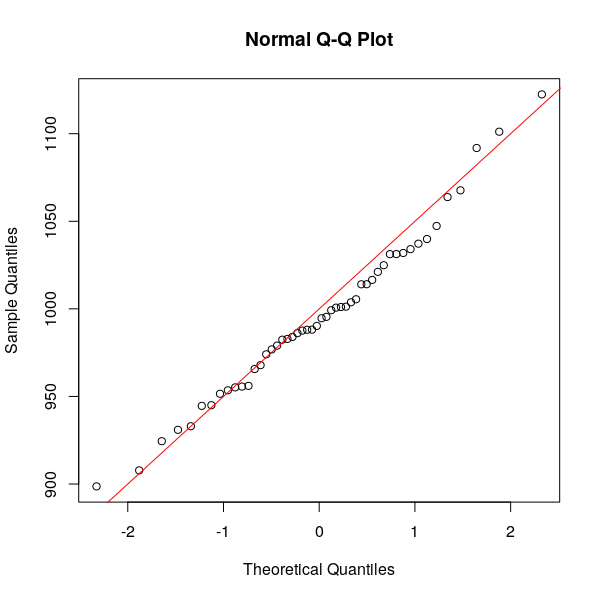
\includegraphics[width=.45\textwidth]{sampling-qqplot-good}
    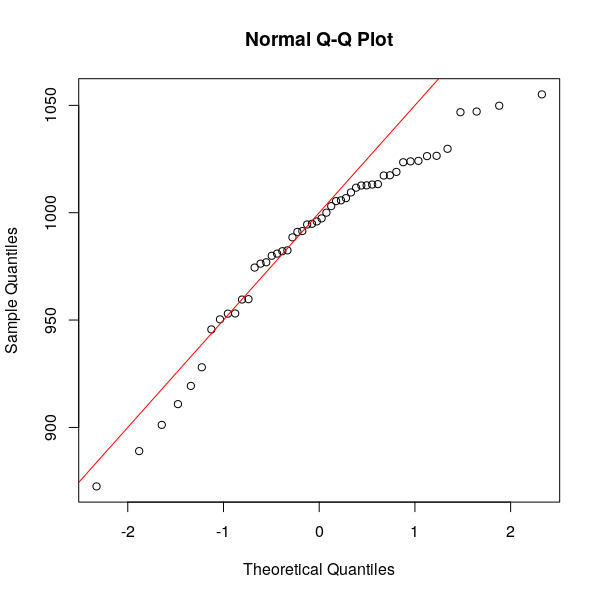
\includegraphics[width=.45\textwidth]{sampling-qqplot-bad}
  \end{center}
  \caption{De QQ-plot links is gebaseerd op een steekproef van 50 observaties uit een normale distributie met gemiddelde 1000 en standaardafwijking 50. De rechterplot is gebaseerd op een Student-$t$ distributie met 15 vrijheidsgraden. Het aantal observaties, gemiddelde en standaardafwijking zijn hetzelfde als links.
    De lijnen in het rood duiden aan waar zich in theorie de observaties zouden moeten bevinden. Links is dat min of meer zo, maar rechts wijken de observaties af, vooral in de extremen.}
  \label{fig:qqplot}
\end{figure}

\lstinputlisting{data/qqplot.R}

\subsection[Chi-kwadraatverdeling]{$\chi^{2}$ verdeling}
Laat $X_{1}, X_{2}, \dots X_{v}$ onafhankelijk standaardnormale variabelen zijn ($\sim N(0,1)$). De $\chi^{2}$ (chi-kwadraat) variabele wordt als volgt gedefinieerd:
\[ \chi^{2}_{v} = X_{1}^{2} + X_{2}^{2} + \dots + X_{v}^{2} \]

Het getal $v$ noemt men het aantal vrijheidsgraden van de variabele. $\chi^{2}$ is een continue toevalsveranderlijke, die positief is omdat ze de som is van kwadraten. Haar dichtheidsfunctie is de volgende:

\[ f_{n}(x) = \frac{1}{2^{\frac{n}{2}}\Gamma(\frac{n}{2})} x^{\frac{n}{2} -1} e^{\frac{x}{2}} \]

De verwachtingswaarde (= gemiddelde) is $v$ en zijn variantie is $2v$. Zijn modus voor $v \geq 2$ is $v-2$.

De $\chi^{2}$ variabele komt niet in de natuur voor. Geen verschijnsel kan erdoor gemodelleerd worden. maar deze variabele zal zeer belangrijk zijn in het vervolg van de cursus.

\section{Centrale limietstelling}
\label{sec:centrale-limietstelling}

\begin{definition}[Lineaire combinatie van onafhankelijke, gelijk verdeelde stochasten]
Formeel: Een lineaire combinatie van onafhankelijke, gelijk verdeelde stochasten is steeds normaal verdeeld.

\[X_{i} \sim Nor(\mu_{i}, \sigma_{i}) \Rightarrow Y = \sum_{i} \alpha_{i} X_{i} \textnormal{ ook normaal verdeeld} \]

Bijgevolg zal ook het steekproefgemiddelde van een steekproef uit een populatie met een willekeurige verdeling, nagenoeg normaal verdeeld zijn voor een voldoende grote $n$.
\end{definition}

Wanneer men dus een aselecte steekproef neemt van onafhankelijke variabelen met een normale verdeling, dan zegt de centrale limietstelling dat het gemiddelde van deze steekproef bij benadering normaal verdeeld zal zijn. Dus als men steeds opnieuw een steekproef neemt met dezelfde grootte, en telkens het gemiddelde optekent, bekomt men bij benadering de grafiek van een normale verdeling. Hoe groter de steekproef, hoe beter de benadering. Het steekproefgemiddelde is dus normaal verdeeld, onafhankelijk van de onderliggende verdeling van de grootheid waarvan men een steekproef neemt. Algemeen kunnen we volgende stelling poneren:

\begin{definition}[Centrale limietstelling]
Beschouw een aselecte steekproef van $n$ waarnemingen die uit een populatie met verwachtingswaarde $\mu$ en standaardafwijking $\sigma$ wordt genomen. Als $n$ groot genoeg is zal de kansverdeling van het steekproefgemiddelde $\overline{x}$ een normale verdeling benaderen met verwachting $\mu_{\overline{x}} = \mu$ en standaardafwijking $\sigma_{\overline{x}} = \frac{\sigma}{\sqrt{n}}$. Hoe groter de steekproef is, des te beter zal de kansverdeling van $\overline{x}$ de verwachtingswaarde van de populatie benaderen.

\end{definition}

Bij het afnemen van een steekproef is zelden de onderliggende verdeling gekend, en toch kan men uitspraken doen over de gemiddelde waarde. Dit is volledig te danken aan de centrale limietstelling, die dit gemiddelde een regel oplegt los van de onderliggende kansverdeling. De centrale limietstelling houdt het steekproefgemiddelde in bedwang, sluit het op in de Gaussische kooi waaruit het nooit kan ontsnappen. Dit, en alleen dit, laat wetenschappers toe het nauwkeurig te bestuderen, te observeren en stelt hen in staat te concluderen.

Want, mocht de verdeling van het steekproefgemiddelde afhankelijk zijn van de onderliggende verdeling, een resultaat dat men tot op zekere hoogte zelfs zou verwachten, zou het onmogelijk zijn om concrete uitspraken te doen over vele wetenschappelijke resultaten. In de theoretische statistiek duiken vrijwel constant limieten van steekproefgemiddeldes op, en deze kunnen dankzij de centrale limietstelling zonder verpinken vervangen worden door een normale verdeling. Zou dit niet mogelijk zijn, dan zou de ganse theorie rond het schatten van parameters in elkaar storten wat dan weer rampzalig zou zijn voor de praktijk. Onderzoeken vergelijken zou herleid worden tot een quasi onmogelijke opgave, en de statistiek in het algemeen zou veel lastiger en ingewikkelder worden.

\subsection{Toepassing van de centrale limietstelling}
Bij het trekken van een aselecte steekproef van omvang $n$ uit een populatie met (onbekend) gemiddelde $\mu$ en standaarddeviatie $\sigma$ is de kansverdeling van het steekproefgemiddelde een kansvariabele $M \sim N (\overline{x}, \frac{\sigma}{\sqrt{n}})$, op voorwaarde dat de steekproefomvang voldoende groot is.

\begin{example}
  We bekijken nu de reactiesnelheid van al onze superhelden en uit onze steekproef met $n = 100$ en $\overline{x} = 90, \sigma = 90$ (miliseconden). Dan kunnen we ons de vraag stellen: wat is de kans dat de gemiddelde reactiesnelheid van een superheld minder is dan $104 ms$?


  \begin{enumerate}
    \item De kansvariabele hier is de gemiddelde reactiesnelheid $\overline{x}$ in een steekproef van $n=100$ superhelden. Daarom geldt wegens de centrale limietstelling:
    \[ \overline{x} \sim Nor(\mu = 90, \sigma_{\overline{x}} = \frac{60}{\sqrt{100}} = 6) \]
    \item We kunnen hierbij de passende $z$-score bepalen:
    \[ z = \frac{104-90}{\frac{60}{\sqrt{100}}} = \frac{104-90}{6} = 2,33 \]
    Dus geldt : $P(\overline{x} < 104) = P(Z < 2,33) = 1 - 0,0099 \approx 0,99$
  \end{enumerate}
\end{example}

\subsection{Schatten van een parameter}
Indien we nu een steekproef onderzoeken, willen uit de berekening op de steekproef een aantal conclusies kunnen trekken met betrekking tot de populatie. We willen bijvoorbeeld de gemiddelde kracht kennen van een superheld of de fractie superhelden die rijk zijn. Als we een schatting geven voor dergelijke onbekende parameter, noemen we dat ook een puntschatter. We gebruiken bijvoorbeeld $\overline{x}$ als schatter om $\mu$ te schatten.

\begin{definition}[puntschatter]
  Een puntschatter voor een populatieparameter is een regel of een formule die ons zegt hoe we uit de steekproef een getal moeten berekenen om de populatieparameter te schatten. Een puntschatter is dus een steekproefgrootheid.
\end{definition}

\subsection{Betrouwbaarheidsinterval populatiegemiddelde bij grote steekproef}

In het geval het schatten van een gemiddelde van een populatie uit een steekproef hebben we totaal geen idee over hoe correct onze schatting is. Daarvoor gaan we op zoek naar een interval waarvan we met een bepaalde zekerheid, bv. 95\%, kunnen zeggen dat het de te schatten karakteristiek bevat.

\begin{definition}[Betrouwbaarheidsinterval]
Een betrouwbaarheidsinterval is een regel of een formule die ons zegt hoe we uit de steekproef een interval moeten berekenen dat de waarde van de parameter met een bepaalde hoge waarschijnlijkheid bevat.
\end{definition}

Een eerste goede schatting voor populatiegemiddelde zou het steekproefgemiddelde zijn:

\[ \overline{x} = \frac{1}{n} \sum_{i} x_{i} \]

Natuurlijk is deze schatting niet de werkelijke waarde van de populatie. Daarom wordt vaak rondom $\overline{x}$ een interval geconstrueerd dat de waarden bevat die aannemelijk zijn voor $\mu$. Hiervoor kunnen we gebruik maken van de centrale limietstelling: het gemiddelde in een te trekken steekproef van omvang $n$ is normaal verdeeld met karakteristieken $\mu$ en $\frac{\sigma}{\sqrt{n}}$.  Als we nu het gemiddelde standaardiseren krijgen we:

\[ Z = \frac{\overline{x} - \mu}{\frac{\sigma}{\sqrt{n}}} \]
 Deze uitdrukking hangt van $\mu$ af maar we weten wel dat deze standaardnormaal verdeeld is. We kunnen daarom getallen $-z$ en $z$ vinden, onafhankelijk van $\mu$, waartussen $Z$ met een voorgeschreven kans $1 - \alpha$ ligt. De betrouwbaarheid $1 - \alpha$ geeft aan hoe betrouwbaar we het interval vinden. We nemen hier $1 - \alpha= 0,95$.

\[P(-z < Z < z) = 1 - \alpha = 0,95 \]

Hieruit halen we dat $\alpha = 0,05$. Door het toepassen van de symmetrieregel weten we dus dat we volgende term moeten berekenen:

\[ P( Z < z) = 0,025 \]

Kijken we in de Z-tabel dan vinden we voor de rechterstaartkans $0,025$ de z-score van $1,96$.

Dus vinden we :

\[ P( -1,96 < \frac{\overline{x} - \mu}{\frac{\sigma}{\sqrt{n}}} < 1,96 ) \]
en dus
\[ P ( \overline{x} -1,96 \frac{\sigma}{\sqrt{n}} <\mu < \overline{x} + 1,96 \frac{\sigma}{\sqrt{n}}) \]

Op die manier kunnen we dus grenzen bepalen die een interval aanduidt waar 95\% kans is dat $\mu$ gevonden wordt. Formeel: als je herhaalde steekproeven zou nemen en telkens op basis van het gerealiseerde steekproefgemiddelde $\overline{x}$ een betrouwbaarheidsinterval zou maken, dan zal bij 95\% van de intervallen $\mu$ binnen de intervalgrenzen liggen.

Opgelet, we gaan er hier van uit dat we de standaarddeviatie van de populatie kennen, wat meestal niet zo is. Indien de steekproef groot genoeg is, kunnen we de steekproefstandaarddeviatie nemen als schatter voor de standaarddeviatie voor de populatie.

\[ P ( \overline{x} -1,96 \frac{\sigma_{\overline{x}}}{\sqrt{n}} < \mu < \overline{x} + 1,96 \frac{\sigma_{\overline{x}}}{\sqrt{n}}) \]


\begin{figure}[t]
\centering
\begin{tikzpicture}
\begin{axis}[
  domain=-3:3, samples=100,
  axis lines*=left, xlabel=$z$,
  every axis y label/.style={at=(current axis.above origin),anchor=south},
  every axis x label/.style={at=(current axis.right of origin),anchor=west},
  height=5cm, width=12cm,
  xtick={-1.96,0,1.96}, ytick=\empty,
  enlargelimits=false, clip=false, axis on top,
  grid = major
  ]
  \addplot [fill=cyan!20, draw=none, domain=-3:3] {gauss(0,1)} \closedcycle;
  \draw [yshift=-0.6cm, latex-latex](axis cs:-1.96,0) -- node [fill=white] {$\sigma$} (axis cs:1.96,0);
\end{axis}
\end{tikzpicture}
\caption{Standaardnormale verdeling die 95\% betrouwbaarheidsinterval aanduidt.}
\label{fig:verdelingStandaardnormaal}
\end{figure}

\subsection{Betrouwbaarheidsinterval populatiegemiddelde bij een kleine steekproef}

Bij kleine steekproeven kunnen we niet langer veronderstellen dat de kansverdeling van $\overline{x}$ bij benadering
normaal verdeel is, omdat de centrale limietstelling alleen normaliteit garandeert voor grote steekproeven ($n >30$). De vorm
van de kansverdeling van het steekproefgemiddelde $\overline{x}$ hangt nu af van de vorm van de verdeling van de populatie waaruit de
steekproef genomen wordt. Alhoewel nog steeds geldt dat $\sigma_{\overline{x}} = \frac{\sigma}{\sqrt{n}}$ kan
de standaardafwijking $s$ een slechte benadering zijn voor $\sigma$ als de steekproef klein is.

Als oplossing kunnen we een nieuwe grootheid bepalen. In plaats van

\[ z = \frac{\overline{x} - \mu}{\frac{\sigma}{\sqrt{n}}} \]

construeren we

\[ t = \frac{\overline{x} - \mu}{\frac{s}{\sqrt{n}}} \]

Deze heeft een kansverdeling die beschreven wordt door een Student-t verdeling. Deze lijkt zeer goed op de normale verdeling: klokvormig, symmetrisch en met verwachtingswaarde 0.

De precieze vorm van de kansverdeling $t$ hang af van de steekproefomvang $n$. We zeggen dat de t-verdeling $(n-1)$ vrijheidsgraden heeft (afgekort $df$).
Merk op dat:
\begin{itemize}
  \item $(n-1)$ ook gebruikt werd om $s^{2}$ te berekenen
  \item als $n \rightarrow \infty$ we de standaardnormale verdeling verkrijgen.
\end{itemize}

Indien we nu een betrouwbaarheidsinterval willen bepalen voor een steekproef met een klein aantal waarden moeten we het volgende doen:

\begin{definition}[Betrouwbaarheidsinterval kleine steekproef]
  Om een betrouwbaarheidsinterval voor het gemiddelde te bepalen op basis van een klein steekproef bepalen we:
  \[ \overline{x} \pm t_{\frac{\alpha}{2}}(\frac{s}{\sqrt{n}}) \]
  waarbij $t_{\frac{\alpha}{2}}$ gebaseerd is op $(n-1)$ vrijheidsgraden. We veronderstellen wel dat we een aselecte steekproef genomen hebben uit
  een populatie die bij benadering normaal verdeeld is.
\end{definition}

\begin{table}
  \centering
  \begin{tabular}{ll}
  	\textbf{Functie} & \textbf{Betekenis}                                             \\ \midrule
  	\verb|pt(x, df)| & Linkerstaartkans, $P(X<\mathtt{x})$                            \\
  	\verb|dt(x, df)| & Hoogte van de curve op punt \texttt{x}                         \\
  	\verb|qt(p, df)| & Onder welke grens zal \texttt{p}\% van de waarnemingen liggen? \\
  	\verb|rt(n, df)| & Genereer \texttt{n} random getallen volgens deze verdeling
  \end{tabular}

  \caption{Kansberekeningsfuncties in R voor de Student-$t$ verdeling met \texttt{df} vrijheidsgraden, verwachte waarde 0 en standaardafwijking 1.}
  \label{tab:t-prob-r}
\end{table}

\subsection{Betrouwbaarheidsinterval voor populatiefractie bij een grote steekproef}

Indien je een variabele wil meten als een fractie, bijvoorbeeld \% mensen die ja geantwoord heeft op een bepaalde vraag, dan willen we in feite de kans $p$ op succes in een binomiaal experiment schatten, waarbij $p$ de kans is dat een willekeurig geselecteerde respondent (of element van de populatie) een succes is (succes in termen van binomiaal experiment). We kunnen $p$ dan schatten door bijvoorbeeld:

\[ \overline{p} = \frac{\textnormal{aantal successen}}{n} \]

Om nu de betrouwbaarheid van de schatter $\overline{p}$ te bepalen moeten we de kansverdeling kennen van $\overline{p}$. Dit kunnen we beredeneren door toepassing van de centrale limietstelling op het gemiddelde aantal successen in de steekproef van omvang $n$. Indien succes = 1 en faling = 0, dan hebben we een steekproef van $n$ elementen, ieder met dezelfde verdeling (kans op 1 is $p$ en kans op 0 is $q=1-p$).  Het gemiddelde $\overline{p}$ heeft dan bij benadering een normale verdeling. Of dus:

\begin{itemize}
  \item Verwachting van kansverdeling van $\overline{p}$ is $p$.
  \item De standaardafwijking van kansverdeling $\overline{p} = \sqrt{\frac{pq}{n}}$
  \item Voor grote steekproeven is $\overline{p}$ bij benadering normaal verdeeld.
\end{itemize}

Aangezien $\overline{p}$ een steekproefgemiddelde is van het aantal successen, stelt dit ons in staat een betrouwbaarheidsinterval te berekenen analoog als die voor de intervalschatting van $\mu$ voor grote steekproeven.

\begin{definition}[Betrouwbaarheidsinterval voor $p$ gebaseerd op grote steekproef]
  \[ \overline{p} \pm z_{\frac{\alpha}{2}} \sqrt{\frac{\overline{p}\overline{q}}{n}} \]
  met $\overline{p} = \frac{x}{n}$ en $\overline{q} = 1- \overline{p}$
\end{definition}

\section{Oefeningen}
\label{sec:steekproefonderzoek-oefeningen}

\begin{exercise}
  Een onderzoeker wil zo correct mogelijk de consumptiegewoontes van de inwoners van 18 jaar en ouder in een bepaalde gemeente, met 3 woonkernen, onderzoeken.  Hij onderscheidt 4 leeftijdsgroepen zodat hij uiteindelijk aan 12 deelgroepen komt. Hij vraagt de procentuele samenstelling van de bevolking op in de gemeente en berekent daaruit hoeveel bevragingen hij per deelgroep moet uitvoeren.  Dit noemen we een \emph{quotasteekproef}.
  
  Vragen:
  \begin{enumerate}[label=\alph*.]
    \item Wat zijn de voor- en nadelen?
    \item Welke soort fouten kunnen hier gemaakt worden?
    \item Welke andere parameters zouden kunnen gebruikt worden bij het opsplitsen in deelgroepen?
  \end{enumerate}
\end{exercise}

\begin{exercise}
  Een onderzoeksbureau wil het aankoopgedrag van wasprodukten nagaan. Men beslist een aantal vragen te stellen aan vrouwen tussen de 25 en 55 jaar omdat men ervan uitgaat dat de relevante populatie uit deze categorie consumenten bestaat. 
  
  Vraag:
  
  \begin{enumerate}[label=\alph*.]
    \item Welke fout wordt hier gemaakt? 
    \item Hoe groot is de impact van deze fout?
  \end{enumerate}
\end{exercise}

\begin{exercise}
  	De vakbonden willen een onderzoek doen naar de werkomstandigheden van de werknemers van een IT-bedrijf. Dat bedrijf heeft in totaal 3200 werknemers die verdeeld zijn over 
  12 vestigingen. Omdat het aantal werknemers groot is worden aselect 40 werknemers gekozen per vestiging. De steekproefomvang is dus $n = 480$.	
  \begin{enumerate}[label=\alph*.]
    \item Welk bezwaar kan tegen deze steekproefprocedure worden gebracht?
    \item Wanneer zou dit geen bezwaar zijn?
  \end{enumerate}
\end{exercise}

\begin{exercise}
  We willen een onderzoek voeren naar onze studenten aan de Hogeschool Gent, faculteit Bedrijf en Organisatie. Hiervoor worden de aanwezige studenten in een bepaald opleidingsonderdeel bevraagd.
  
  \begin{enumerate}[label=\alph*.]
    \item Welke kritiek kan je op deze methode geven?
    \item Stel dat de aanwezige docent een kernvak geeft, zeer streng is en tijdens de bevraging rondloopt. Welk bezwaar kan hier gegeven worden?
    \item Stel dat de bevraging niet tijdens een les, maar na een examen gehouden wordt. Welke kritiek kan je op deze methode geven?
  \end{enumerate}
\end{exercise}

\begin{exercise}
  Bereken met behulp van de tabel van de normale verdeling de volgende kansen door de gevraagde kans te herleiden tot een linkerstaartkans. Teken ook elke keer het gevraagde gebied.
  \begin{enumerate}[label=\alph*.]
    \item $P(Z < 1.33)$
    \item $P(Z > 1.33)$
    \item $P(Z < -1.33)$
    \item $P(Z > -1.33)$
    \item $P(Z < 0.45)$
    \item $P(Z > -1.05)$
    \item $P(Z < 0.65)$
    \item $P(-0.45 < Z < 1.20)$
    \item $P(-1.35 < Z < -0.10)$
    \item $P(-2.10 < Z < -0.90)$
  \end{enumerate}
\end{exercise}

\begin{exercise}
  In de  Hogeschool zijn er twee klassen voor het vak onderzoekstechnieken. De studenten werden willekeurig over de klassen verdeeld, zodat we mogen veronderstellen dat de ene klas niet slimmer is dan de andere. In de A-klas geeft mevr. X les, in de B-klas geeft mr. Y les. X is nogal streng en op het einde van het schooljaar behaalt haar klas een gemiddelde van 54 op 100 met een standaardafwijking van 11.

  Y is iets losser en stimuleert de leerlingen al gauw met een puntje meer. Op het einde van het schooljaar behaalt zijn klas een gemiddelde van 62 op 100 en een standaardafwijking van 7.

  Wouter zit in de A-klas en heeft $\frac{63}{100}$ voor wiskunde. Stijn zit in de B-klas en behaalt $\frac{67}{100}$. Wie heeft volgens jou het beste gescoord?
\end{exercise}

\begin{exercise}
  Een gezondheidsonderzoek tussen 1988 en 1994 gaf aan dat de gemiddelde cholesterolwaarde bij vrouwen tussen 20 en 29 jaar 183 mg/dl bedroeg, met een standaardafwijking gelijk aan 36. We nemen nu een aselecte steekproef van 81 vrouwen. Los volgende vragen op:
  
  \begin{enumerate}[label=\alph*.]
    \item Schets de kansdichtheidsfunctie voor de populatie en de kansverdeling van het steekproefgemiddelde $\overline{x}$.
    \item Bepaald de kans dat $\overline{x}$ kleiner is dan 185.
    \item Bepaal de kans dat $\overline{x}$ tussen 175 en 185 ligt.
    \item Bepaal de kans dat $\overline{x}$ groter is dan 190. 
  \end{enumerate}
\end{exercise}

\begin{exercise}
  Een aselecte steekproef van 64 stuks wordt getrokken uit een populatie met onbekende verdeling. De verwachting en de standaardafwijking van de populatie
  zijn wel gekend: $\mu = 20$ en $\sigma=16$. Los volgende vragen op:
  
  \begin{enumerate}[label=\alph*.]
    \item Bepaal de verwachting en standaardafwijking van het steekproefgemiddelde.
    \item Beschrijf de vorm van de verdeling van het steekproefgemiddelde. In hoeverre hangt je antwoord af van de grootte van de steekproef?
    \item Bereken de $z$ score bij $\overline{x_{1}} = 15.5$ en $\overline{x_{2}} = 23$.
    \item Bepaal kans dat $\overline{x} <16$.
    \item Bepaal kans dat $\overline{x} > 23$.
    \item Bepaal kans dat $16< \overline{x}< 22$.
  \end{enumerate}
\end{exercise}

\begin{exercise}
  Verkeersdrempels zijn bedoeld om de snelheid van automobilisten te be\"invloeden. Afhankelijk van de gewenste snelheid in een straat worden de drempels steiler of minder steil gemaakt. Drempel A is zo ontworpen dat 85 \% van de automobilisten de drempel passeert met een snelheid van minder dan 50 km per uur. In de praktijk blijkt dat de passeersnelheid bij een drempel normaal verdeeld is. Bij drempel A werd een gemiddelde passeersnelheid van 43,1 km/h gevonden met standaardafwijking 6,6 km/h.
  
  \begin{enumerate}[label=\alph*.]
    \item Toon aan dat 85\% van de automobilisten niet harder dan 50 km/h rijdt.
    \item Bij hoeveel van de 1200 metingen kan, op grond van eerdere ervaringen, een snelheid van meer dan 55 km/h worden verwacht?
  \end{enumerate}
\end{exercise}

\begin{exercise}
  Gegeven 20 examenresultaten in Tabel~\ref{tab:examen}. Uit resultaten van de laatste jaren blijkt dat $\sigma = 2.45$.
  
  \begin{enumerate}[label=\alph*.]
    \item Wat is $\sigma_{\overline{x}}$ , de standaardafwijking van $\overline{x}$?
    \item Geef het 92\% betrouwbaarheidsinterval voor $\mu$.
    \item Kunnen we er zeker van zijn dat het gemiddeld resultaat minder dan 12.5 bedraagt?
  \end{enumerate}
\end{exercise}

\begin{table}
  \centering
  \begin{tabular}{llllllllll}
    11.5 & 16.5 & 11 & 17.3 & 10.8 & 5.6  & 13.1 & 11.5 & 14.2 & 12.9 \\
    8.7  & 9.2  & 15 & 14.4 & 10   & 10.3 & 18.3 & 12.9 & 14.2 & 8.7 
  \end{tabular}
  \caption{Examenresultaten}
  \label{tab:examen}
\end{table}

\begin{exercise}
  Een schoenhandelaar voert een marktonderzoek uit bij 500 klanten. Daaruit blijkt dat 30\% van hen minstens éénmaal per jaar sportschoenen koopt.  Op basis van secundaire informatie weet hij dat het nationaal gemiddelde op 26\% ligt.  Hij vraagt zich nu af in hoeverre zijn zaak in dat opzicht afwijkt van de nationale norm? (We werken met $\alpha= 5\%$, tweezijdig.)
\end{exercise}

\begin{exercise}
  Een conservenfabrikant krijgt de laatste tijd klachten over de netto inhoud van zijn conserven met wortelen en erwtjes, die volgens de verpakking netto 1 liter zouden moeten bevatten. Daarom laat hij een steekproef nemen waarin de netto inhoud van 40 willekeurig gekozen blikjes wordt gecontroleerd. De resultaten worden samengevat in Tabel~\ref{tab:Steekproefwaarden}.

Vraag A: 
\begin{itemize}
  \item Vul de tabel aan met de cummulatieve absolute frequentie
  \item Vul de tabel aan met de relatieve frequentie
  \item Vul de tabel aan met de cummulatieve relatieve frequentie.
\end{itemize}
Vraag B:

\begin{itemize}
  \item Bereken het gemiddelde
  \item Bereken de standaardafwijking
  \item Hoeveel procent van de blikken bevatten te weinig wortelen en erwtjes.
  \item Teken een histogram van de absolute frequentie.
  \item Zijn de gegevens normaal verdeeld?  Hoe zie je dat?
\end{itemize}

\end{exercise}

  \begin{table}
  \centering
  \begin{tabular}{lr}
    \toprule
    Inhoud & $n_{i}$ \\
    \midrule
    $[970,980[$ & 3 \\
    $[980,990[$ & 5 \\
    $[990,1000[$ & 13 \\
    $[1000,1010[$ & 11 \\ 
    $[1010,1020[$ & 5 \\
    $[1020,1030[$ & 3 \\
    \bottomrule
  \end{tabular}
  \caption{Steekproefwaarden}
  \label{tab:Steekproefwaarden}
\end{table}